\documentclass[a4paper, 2pt, landscape]{extarticle}
\usepackage[utf8]{inputenc}
\usepackage[T1]{fontenc}
\usepackage{amsmath, amssymb, bm}
\usepackage{geometry}
\geometry{left=2mm, right=2mm, top=2mm, bottom=2mm}
\usepackage{tikz}
\usetikzlibrary{arrows.meta}
\usepackage{tcolorbox}
\usepackage{multicol}

\definecolor{boxtitle}{RGB}{30,80,150}
\definecolor{col2}{RGB}{210,240,215}  % grün – A2
\definecolor{col3}{RGB}{255,235,200}  % orange – A3
\definecolor{col4}{RGB}{235,215,240}  % lila – A4
\definecolor{col5}{RGB}{255,225,215}  % rot – A5

\tcbset{
  boxrule=0.3pt, arc=1.2pt,
  fonttitle=\bfseries\tiny\color{white},
  coltitle=white, colbacktitle=boxtitle,
  top=1.5pt, bottom=1.5pt, left=2pt, right=2pt,
  toptitle=1pt, bottomtitle=1pt,
  parbox=false
}

\setlength{\parindent}{0pt}
\setlength{\columnsep}{4mm}
\setlength{\abovedisplayskip}{1pt}
\setlength{\belowdisplayskip}{1pt}

\begin{document}
\fontsize{3pt}{4pt}\selectfont

\begin{center}
  \textbf{\small Formelsammlung Elektromagnetische Felder}
\end{center}
\vspace{-2pt}

\begin{multicols*}{5}

% ─────────────────────────────────────────────
\begin{tcolorbox}[title={A2: Kreisbogen}, colback=col2, colframe=boxtitle]
\textbf{Geometrie:} Halbkreisbogen, $\rho \in [\rho_i, \rho_a]$, Breite $b$. Potential $\phi(\rho)$ hängt nur von $\rho$ ab. \\
\textbf{a) Potential:} Laplace: $\frac{1}{\rho}\frac{d}{d\rho}(\rho\frac{d\phi}{d\rho}) = 0$. \\
1. Integration: $\rho \phi' = C_1 \Rightarrow \phi' = C_1/\rho$. 2. Integration: $\phi(\rho) = C_1 \ln \rho + C_2$. \\
RB: $\phi(\rho_i)=\phi_i, \phi(\rho_a)=\phi_a \Rightarrow C_1 = \frac{\phi_a-\phi_i}{\ln(\rho_a/\rho_i)}, C_2 = \phi_i - C_1 \ln \rho_i$. \\
$\boxed{\phi(\rho) = \phi_i + (\phi_a-\phi_i) \frac{\ln(\rho/\rho_i)}{\ln(\rho_a/\rho_i)}}$ \\
\textbf{b) Stromdichte:} $\vec{J} = -\kappa \nabla \phi = -\kappa \frac{d\phi}{d\rho} \vec{e}_\rho = \frac{\kappa(\phi_i-\phi_a)}{\rho \ln(\rho_a/\rho_i)} \vec{e}_\rho$. \\
\textbf{c) Widerstand:} $I = \int \vec{J} \cdot d\vec{A} = \int_0^b \int_0^\pi J(\rho) \rho \, d\varphi \, dz = \frac{\kappa \pi b (\phi_i-\phi_a)}{\ln(\rho_a/\rho_i)}$. \\
$\boxed{R = U/I = \frac{\ln(\rho_a/\rho_i)}{\kappa \pi b}}$ (Halbkreis $\Rightarrow \Delta\varphi = \pi$).
\end{tcolorbox}

% ─────────────────────────────────────────────
\begin{tcolorbox}[title={A3: Biot-Savart}, colback=col3, colframe=boxtitle]
\textbf{Gesetz:} $\vec{B}(\vec{r}) = \frac{\mu_0 I}{4\pi} \oint \frac{d\vec{s}' \times (\vec{r}-\vec{r}')}{|\vec{r}-\vec{r}'|^3}$ \\
\textbf{a) Herleitung Kreis 1 ($R_1$) auf Z-Achse:} \\
Aufpunkt: $\vec{r} = z \vec{e}_z$. Leiterkurve: $\vec{r}' = R_1 \vec{e}_\rho(\varphi) = R_1(\cos\varphi \vec{e}_x + \sin\varphi \vec{e}_y)$. \\
Wegelement (Ableitung): $d\vec{s}' = \frac{d\vec{r}'}{d\varphi} d\varphi = R_1(-\sin\varphi \vec{e}_x + \cos\varphi \vec{e}_y) d\varphi = R_1 \vec{e}_\varphi d\varphi$. \\
Abstand: $\vec{R} = z \vec{e}_z - R_1 \vec{e}_\rho$, Betrag $R = \sqrt{R_1^2+z^2}$. \\
Kreuzprodukt: $d\vec{s}' \times \vec{R} = (R_1 \vec{e}_\varphi d\varphi) \times (z \vec{e}_z - R_1 \vec{e}_\rho) = R_1 z d\varphi \vec{e}_\rho + R_1^2 d\varphi \vec{e}_z$. \\
$\vec{e}_\rho$-Term verschwindet bei Integration $\int_0^{2\pi} d\varphi$ wegen Symmetrie. \\
$\vec{B}_1(z) = \frac{\mu_0 I_1}{4\pi} \int_0^{2\pi} \frac{R_1^2 d\varphi}{(R_1^2+z^2)^{3/2}} \vec{e}_z = \frac{\mu_0 I_1 R_1^2 \cdot 2\pi}{4\pi (R_1^2+z^2)^{3/2}} \vec{e}_z \Rightarrow \boxed{\vec{B}_1(z) = \frac{\mu_0 I_1 R_1^2}{2(R_1^2+z^2)^{3/2}} \vec{e}_z}$ \\
\textbf{b) Superposition:} $\vec{B}_G(z) = \vec{B}_1(z, I_1, R_1) + \vec{B}_2(z, I_2, R_2)$. \\
\textbf{c) $B_G(0)=0$:} $\frac{\mu_0}{2} (\frac{I_1}{R_1} + \frac{I_2}{R_2}) = 0 \Rightarrow \boxed{I_2 = -\frac{R_2}{R_1} I_1}$ (Stromrichtung entgegen).
\end{tcolorbox}
% ─────────────────────────────────────────────
\begin{tcolorbox}[title={A4: Geschichtet}, colback=col4, colframe=boxtitle]
\textbf{Geom:} $a \times a$, Länge $l$, 4 Quadranten parallel. \\
$\kappa_1=\kappa, \kappa_2=2\kappa, \kappa_3=3\kappa, \kappa_4=4\kappa$. \\
\textbf{a) E-Feld \& Potential:} $J = I/A_{ges}, J = \kappa_{ges} E$. \\
$E = -\frac{d\phi}{dx} \Rightarrow \phi = \int -E \,dx$. Da parallel: $E$ überall gleich. \\
$E = \frac{I}{\frac{a^2}{4}(\kappa_1 + \kappa_2 + \kappa_3 + \kappa_4)} \Rightarrow E = \frac{2 \cdot I}{5\kappa a^2}$ 
$\phi(x) - \phi(0) = \int_{l=0}^{x} -E dx \Rightarrow \phi(x) = \phi_0 - \frac{2 \cdot I}{5\kappa a^2} \cdot x $\\
\textbf{b) Widerstand:} $R = U/I \Rightarrow U = \phi(0) - \phi(l) \Rightarrow U = - \frac{2 \cdot I}{5\kappa a^2} \cdot l  \Rightarrow R = \frac{2l \cdot I}{a^2 \cdot 5\kappa \cdot I} = \frac{2l}{5\kappa a^2} $\\
\textbf{c) ESB:} $R_1 \parallel R_2 \parallel R_3 \parallel R_4$ \\
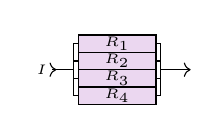
\begin{tikzpicture}[scale=0.55, font=\tiny]
  \draw (0,0.3) -- (0.4,0.3) -- (0.4,0.9) -- (2.4,0.9) -- (2.4,0.3) -- (2.8,0.3);
  \draw (0,0.3) -- (0.4,0.3) -- (0.4,0.5) -- (2.4,0.5) -- (2.4,0.3) -- (2.8,0.3);
  \draw (0,0.3) -- (0.4,0.3) -- (0.4,0.1) -- (2.4,0.1) -- (2.4,0.3) -- (2.8,0.3);
  \draw (0,0.3) -- (0.4,0.3) -- (0.4,-0.3) -- (2.4,-0.3) -- (2.4,0.3) -- (2.8,0.3);
  \draw[fill=col4] (0.5,0.7) rectangle (2.3,1.1) node[pos=.5]{$R_1$};
  \draw[fill=col4] (0.5,0.3) rectangle (2.3,0.7) node[pos=.5]{$R_2$};
  \draw[fill=col4] (0.5,-0.1) rectangle (2.3,0.3) node[pos=.5]{$R_3$};
  \draw[fill=col4] (0.5,-0.5) rectangle (2.3,-0.1) node[pos=.5]{$R_4$};
  \draw[->] (-0.1,0.3) -- (0,0.3) node[left]{$I$};
  \draw[->] (2.8,0.3) -- (3.1,0.3);
\end{tikzpicture}
\end{tcolorbox}

% ─────────────────────────────────────────────
\begin{tcolorbox}[title={A5: Induktion}, colback=col5, colframe=boxtitle]
\textbf{Gegeben:} $i(t) = I_0 \sin(\omega t)$, Linienleiter auf Achsen. \\
\textbf{a) B-Feld:} $H = I/(2\pi r) \Rightarrow \vec{B}_y = -\frac{\mu_0 i}{2\pi x} \vec{e}_z, \vec{B}_x = \frac{\mu_0 i}{2\pi y} \vec{e}_z$. \\
$\vec{B}(x,y) = \frac{\mu_0 i(t)}{2\pi} (\frac{1}{y} - \frac{1}{x}) \vec{e}_z$. \\
\textbf{b) Spannung:} $U_{ind} = -\dot{\Phi}$. Fluss $\Phi = \iint B dA$. \\
$\Phi = \frac{\mu_0 i(t)}{2\pi} \int_{x_0}^{x_0+b} \int_{y_0}^{y_0+h} (\frac{1}{y} - \frac{1}{x}) dy dx$. \\
$\Phi = \frac{\mu_0 i(t)}{2\pi} [b \ln \frac{y_0+h}{y_0} - h \ln \frac{x_0+b}{x_0}]$. \\
{\raggedright
$U_{ind} = -\frac{\mu_0 \omega I_0 \cos \omega t}{2\pi} [b \ln \frac{y_0+h}{y_0} - h \ln \frac{x_0+b}{x_0}]$ \par}
\end{tcolorbox}

\begin{tcolorbox}[title={Kreisbogen \normalfont(azimutal entlang des bogens ($\phi$))}, colback=col2, colframe=boxtitle]
\textbf{Geometrie:} Halbkreisbogen, $\rho \in [\rho_i, \rho_a]$, Breite $b$. Potential $\phi(\varphi)$ hängt nur von $\varphi$ ab. \\
\textbf{a) Potential:} Laplace: $\Delta \phi = 0 \Rightarrow \frac{1}{\rho^2} \frac{d^2\phi}{d\varphi^2} = 0$. \\
Integrationen: $\phi'(\varphi) = C_1 \Rightarrow \phi(\varphi) = C_1 \cdot \varphi + C_2$. \\
RB: $\phi(0)=\phi_a, \phi(\pi)=\phi_b \Rightarrow C_2 = \phi_a, C_1 = \frac{\phi_b-\phi_a}{\pi}$. \\
$\boxed{\phi(\varphi) = \frac{\phi_b-\phi_a}{\pi} \cdot \varphi + \phi_a}$ \\
\textbf{b) Stromdichte:} $\vec{E} = -\nabla \phi = -\frac{1}{\rho} \frac{d\phi}{d\varphi} \vec{e}_\varphi = -\frac{1}{\rho} \cdot \frac{\phi_b-\phi_a}{\pi} \vec{e}_\varphi$. \\
$\vec{J} = \kappa \vec{E} = -\frac{\kappa}{\rho} \cdot \frac{\phi_b-\phi_a}{\pi} \vec{e}_\varphi = \frac{\kappa(\phi_a-\phi_b)}{\pi \rho} \vec{e}_\varphi$. \\
\textbf{c) Widerstand:} $I = \iint \vec{J} \cdot d\vec{A} = \int_{z=0}^b \int_{\rho=\rho_i}^{\rho_a} \frac{\kappa(\phi_a-\phi_b)}{\pi \rho} \, d\rho \, dz = \frac{\kappa \cdot b \cdot (\phi_a-\phi_b)}{\pi} \ln\left(\frac{\rho_a}{\rho_i}\right)$. \\
$U = \phi_a - \phi_b \Rightarrow R = U/I = \frac{\phi_a-\phi_b}{\frac{\kappa \cdot b \cdot (\phi_a-\phi_b)}{\pi} \ln(\rho_a/\rho_i)} = \boxed{\frac{\pi}{\kappa \cdot b \cdot \ln(\frac{\rho_a}{\rho_i})}}$.
\end{tcolorbox}

% ─────────────────────────────────────────────
\begin{tcolorbox}[title={Nützliche Laplace-Lösungen}, colback=white, colframe=boxtitle]
\textbf{Kartesisch ($\phi(x)$):} $\phi''=0 \Rightarrow \phi = C_1 x + C_2$ \\
\textbf{Zylinder ($\phi(\rho)$):} $(\rho \phi')' = 0 \Rightarrow \phi = C_1 \ln \rho + C_2$ \\
\textbf{Zylinder ($\phi(\varphi)$):} $\phi''=0 \Rightarrow \phi = C_1 \varphi + C_2$ \\
\textbf{Kugel ($\phi(r)$):} $(r^2 \phi')' = 0 \Rightarrow \phi = C_1/r + C_2$ \\
\textbf{Kugel ($\phi(\theta)$):} $\phi = C_1 \ln(\tan \frac{\theta}{2}) + C_2$ \\
\textbf{Gradient (Zyl):} $\nabla \phi = \partial_\rho \phi \vec{e}_\rho + \frac{1}{\rho} \partial_\varphi \phi \vec{e}_\varphi + \partial_z \phi \vec{e}_z$ \\
\textbf{Fluss:} $\Phi = \int \vec{B} \cdot d\vec{A}$. \textbf{Induktion:} $U_{ind} = -\frac{d\Phi}{dt}$ \\
$\hat{e}_\rho \times \hat{e}_\varphi = \hat{e}_z$; $\hat{e}_\varphi \times \hat{e}_z = \hat{e}_\rho$; $\hat{e}_z \times \hat{e}_\rho = \hat{e}_\varphi$ \\
\textbf{Konstanten:} $\mu_0 = 4\pi \cdot 10^{-7}$ H/m.
\end{tcolorbox}

% --- GRUPPE 1: ANALYSIS ---
\begin{tcolorbox}[title={Vektoranalysis \& Grundlagen (B1 \& B10)}]
\textbf{Operatoren (Ortsvektor $\vec{r}$):} \\
$\nabla r = \frac{\vec{r}}{r}$; \quad $\nabla \frac{1}{r} = -\frac{\vec{r}}{r^3}$ \\
$\text{div } \vec{r} = 3$; \quad $\text{div } \frac{\vec{r}}{r} = \frac{2}{r}$; \quad $\text{div } \frac{\vec{r}}{r^3} = 0$ \\
$\text{rot } \vec{r} = \vec{0}$; \quad $\text{rot } (f(r)\vec{r}) = \vec{0}$ \\
\textbf{Potentialbestimmung:} \\
$\vec{F} = -\nabla \phi \Rightarrow \phi = -\int \vec{F} \cdot d\vec{s}$ \\
Bsp: $\vec{F}=(2xy^3z^4+2)\vec{e}_x + \dots \Rightarrow \phi = -(x^2y^3z^4+2x)$ \\
\textbf{Einheiten:} $[D] = \text{C/m}^2$; $[H] = \text{A/m}$; $[B] = \text{T} = \text{Vs/m}^2$
\end{tcolorbox}

% --- GRUPPE 2: ELEKTROSTATIK ---
\begin{tcolorbox}[title={Elektrostatik (B1, B3, B4)}]
\textbf{Kugelladung (homogen, Radius $R$):} \\
$r \le R: \vec{E} = \frac{Q \cdot r}{4\pi\epsilon_0 R^3} \vec{e}_r$; \quad $\phi = \frac{\rho_V}{6\epsilon}(3R^2 - r^2)$ \\
$r > R: \vec{E} = \frac{Q}{4\pi\epsilon_0 r^2} \vec{e}_r$; \quad $\phi = \frac{\rho_V R^3}{3\epsilon r}$ \\
\textbf{Linienladung:} $\phi(\rho) = -\frac{\rho_L}{2\pi\epsilon_0} \ln(\frac{\rho}{\rho_0})$ \\
\textbf{Kreisscheibe (z-Achse):} $\phi(z) = \frac{\rho_F}{2\epsilon_0}(\sqrt{R^2+z^2}-|z|)$ \\
\textbf{Kondensatoren:} \\
Koaxial: $C = \frac{2\pi\epsilon l}{\ln(b/a)}$; \quad $\phi(\rho) = \frac{\phi_a-\phi_b}{\ln(b/a)}\ln(\frac{\rho}{b}) + \phi_b$ \\
Kugel: $C = 4\pi\epsilon \frac{ab}{b-a}$; \quad $\vec{E} = \frac{U}{r^2}\frac{ab}{b-a}\vec{e}_r$ \\
\textbf{Spiegelung (Linienladung $h$ über Boden):} \\
$\phi(x,z) = \frac{\rho_L}{2\pi\epsilon} \ln \frac{\sqrt{x^2+(z+h)^2}}{\sqrt{x^2+(z-h)^2}}$
\end{tcolorbox}

% --- GRUPPE 3: STRÖMUNGSFELDER ---
\begin{tcolorbox}[title={Strömungsfelder \& Widerstände (B5, B8)}]
\textbf{Lösungsalgorithmus:} $\vec{J} = \frac{I}{A} \to \vec{E} = \frac{\vec{J}}{\kappa} \to U = \int \vec{E} d\vec{s} \to R = \frac{U}{I}$ \\
\textbf{Geschichtete Medien:} \\
Reihe (I konst): $\vec{E}_i = \frac{I}{\kappa_i A}$; \quad $\phi(x)$ stückweise linear \\
Zylinder (vertikal): $R = \frac{\ln(\rho_a/\rho_i)}{2\pi(l_1\kappa_1 + l_2\kappa_2)}$ \\
\textbf{Spezialformen:} \\
Kegel: $A(x) = A_0(x\frac{\alpha-1}{l}+1) \to R = \frac{\ln \alpha}{\kappa A_0 (\alpha-1)}$ \\
Kugel ($\kappa = \kappa_0 \frac{a}{r}$): $R = \frac{1}{4\pi\kappa_0 a} \ln(\frac{r_a}{r_i})$ \\
Halbkreisbogen: $R = \frac{\pi}{b \kappa \ln(\rho_a/\rho_i)}$; \quad $\phi(\varphi) = \frac{\phi_b-\phi_a}{\pi}\varphi + \phi_a$ \\
\textbf{Erdung (Halbkugel):} $\phi(r) = \frac{I}{2\pi\kappa r}$; \quad $R_E = \frac{1}{2\pi\kappa a}$ \\
\textbf{Schrittspannung:} $U_{SZ} \approx E \cdot s$; \quad max bei $x_m = a/\sqrt{2}$
\end{tcolorbox}

% --- GRUPPE 4: MAGNETOSTATIK ---
\begin{tcolorbox}[title={Magnetostatik \& Biot-Savart (B6, B8)}]
\textbf{Biot-Savart Felder:} \\
Unendl. Leiter: $\vec{B} = \frac{\mu_0 I}{2\pi \rho} \vec{e}_\varphi$ \\
Leiterstück ($0 \le x \le \infty$): $\vec{H} = -\frac{I}{4\pi R} \vec{e}_z$ \\
Leiterstück ($0 \le x \le R$): $\vec{H} = -\frac{I}{4\pi R \sqrt{2}} \vec{e}_z$ \\
Viertelkreisbogen: $\vec{H} = -\frac{I}{8R} \vec{e}_z$ \\
Kreisring (Achse $x$): $\vec{H}(x) = \frac{I R^2}{2(R^2+x^2)^{3/2}} \vec{e}_x$ \\
Quadratische Schleife (Achse $z$): $\vec{H} = \frac{I}{\pi} \frac{a^2}{(\frac{a^2}{2}+z^2)\sqrt{a^2+z^2}} \vec{e}_z$ \\
Spiralschleife (Ursprung): $\vec{H} = \frac{1}{2a} \ln(3) \vec{e}_z$ \\
Stromschiene: $\vec{H} = \frac{I}{\pi h} \arctan(\frac{h}{2x}) \vec{e}_y$ \\
\textbf{Energie:} $W_m = \frac{\mu_0 I^2 l}{4\pi} \ln \frac{b}{a}$
\end{tcolorbox}

% --- GRUPPE 5: INDUKTION ---
\begin{tcolorbox}[title={Induktion (B7, B8)}]
\textbf{Gesetz:} $U_{ind} = -\frac{d\Phi}{dt}$ \\
\textbf{Konfigurationen:} \\
Ruhend ($i(t)$): $U_{ind} = -\frac{\mu_0 I_0 \omega h}{2\pi} \ln \frac{y_0+b}{y_0} \cos(\omega t)$ \\
Bewegt ($\vec{v}$, $I$ konst): $U_{ind} = \frac{\mu_0 I_0 v_0 h}{2\pi} \frac{b}{(y_0+v_0 t)(y_0+v_0 t+b)}$ \\
Kombiniert ($i(t)$ \& $\vec{v}$): Summe aus Trafo- und Bewegungsterm \\
Rotation ($H_0$): $U_{ind} = 4ab \mu_0 H_0 \omega \sin(\omega t)$ \\
2 Leiter \& Schleife: $u_{ind}(t) = -\mu_0 \frac{b I_0 \omega}{2\pi} \cos(\omega t) \ln \left( \frac{(x_0+a)(x_0+a-c)}{x_0(x_0-c)} \right)$
\end{tcolorbox}

\begin{tcolorbox}[title={Herleitung: Punktladung im Vakuum}, colback=white, colframe=boxtitle]
\textbf{Elektrische Feldstärke $\vec{E}$ (Gaußsches Gesetz)} \\
Ausgangspunkt ist das Gaußsche Gesetz in Integralform. Wir wählen als Integrationsfläche $A$ eine konzentrische Kugelfläche mit Radius $r$ um die Punktladung $Q$.
$\oint_{A} \vec{D} \cdot d\vec{A} = Q \quad \text{mit} \quad \vec{D} = \varepsilon_0 \vec{E}$
Aufgrund der Kugelsymmetrie steht $\vec{E}$ überall senkrecht auf der Fläche und der Betrag $E$ ist konstant auf der Hülle:
$\varepsilon_0 E \cdot \underbrace{4\pi r^2}_{\text{Kugeloberfläche}} = Q \implies E(r) = \frac{Q}{4\pi\varepsilon_0 r^2}$
Vektoriell mit dem radialen Einheitsvektor $\vec{e}_r$:
$\vec{E}(\vec{r}) = \frac{Q}{4\pi\varepsilon_0 r^2} \vec{e}_r$
\end{tcolorbox}

\begin{tcolorbox}[title={Geschichtete Medien I (Reihe) Dielektrikum ist nacheinander}, colback=white, colframe=boxtitle]
Das Feld steht senkrecht auf der Grenzfläche, weshalb die Flussdichte $\vec{D}$ stetig ist. 

In beiden Medien gilt: $\vec{D}_1 = \vec{D}_2 = \rho_A \vec{e}_x$

Die elektrischen Feldstärken berechnen sich zu: 
$\vec{E}_1 = \frac{\rho_A}{\epsilon} \vec{e}_x$ \quad und \quad $\vec{E}_2 = \frac{\rho_A}{2\epsilon} \vec{e}_x$

Mit der Randbedingung $\phi(d_2) = 0$ ergibt sich der Potentialverlauf:
Für $d_1 \le x \le d_2$: \quad $\phi_2(x) = \frac{\rho_A}{2\epsilon} (d_2 - x)$
Für $0 \le x \le d_1$: \quad $\phi_1(x) = \frac{\rho_A}{\epsilon} (d_1 - x) + \frac{\rho_A}{2\epsilon} (d_2 - d_1)$

Da $\vec{E}_1 = 2\vec{E}_2$, ist die Feldliniendichte von $\vec{E}$ in Medium 1 doppelt so hoch. 
Die Anordnung entspricht einer Reihenschaltung: $C_1 = \frac{\epsilon A}{d_1}$ und $C_2 = \frac{2\epsilon A}{d_2 - d_1}$
\end{tcolorbox}

\begin{tcolorbox}[title={Lösung Aufgabe 4: Geschichtete Medien II (Parallel) Dielektrikum ist übereinander}, colback=white, colframe=boxtitle]
Das Feld verläuft parallel zur Grenzfläche, wodurch die Feldstärke $\vec{E}$ identisch bleibt.

In beiden Medien gilt: $\vec{E}_1 = \vec{E}_2 = \frac{U}{d} \vec{e}_x$

Die zugehörigen Flussdichten berechnen sich zu:
$\vec{D}_1 = \epsilon \frac{U}{d} \vec{e}_x$ \quad und \quad $\vec{D}_2 = 2\epsilon \frac{U}{d} \vec{e}_x$

Der Potentialverlauf ist für beide Schichten gleich: $\phi(x) = \frac{U}{d} (d - x)$

Über die Gesamtladung $Q = \rho_A A = D_1 A_1 + D_2 A_2$ folgt für die Spannung:
$U = \frac{\rho_A A d}{\epsilon A_1 + 2\epsilon A_2}$

Die $\vec{D}$-Linien sind in Medium 2 doppelt so dicht wie in Medium 1. 
Die Anordnung entspricht einer Parallelschaltung: $C_1 = \frac{\epsilon A_1}{d}$ und $C_2 = \frac{2\epsilon A_2}{d}$
\end{tcolorbox}

% --- AUFGABE 2: STRÖMUNGSFELD KEGEL ---
\begin{tcolorbox}[title={Aufgabe 2: Strömungsfeld Kegel (Blatt 5)}]
\textbf{Frage:} Ein Medium mit Leitfähigkeit $\kappa$ hat einen linear veränderlichen Querschnitt $A(x)$. Gesucht sind $A(x)$, $E(x)$, der Potentialverlauf $\phi(x)$ und der Widerstand $R$.

\textbf{Lösung:}
Der Querschnitt ändert sich linear von $A_0$ zu $\alpha A_0$: 
$A(x) = A_0 (1 + \frac{\alpha - 1}{l} x)$.

Die Feldstärke ergibt sich aus $J = I/A(x)$: 
$E(x) = \frac{I}{\kappa A_0 (1 + \frac{\alpha - 1}{l} x)}$.

Das Potential berechnet sich durch Integration mit $\phi(0) = 0$: \\
$\phi(x) = -\int_{0}^{x} E(x') dx' = -\frac{I \cdot l}{\kappa A_0 (\alpha - 1)} \ln(1 + \frac{\alpha - 1}{l} x)$.

Der Widerstand folgt aus $R = \frac{|\phi(l)|}{I}$: 
$R = \frac{l}{\kappa A_0 (\alpha - 1)} \ln(\alpha)$.
\end{tcolorbox}

% --- AUFGABE 1: GESCHICHTETES MEDIUM ---
\begin{tcolorbox}[title={Aufgabe 1: Geschichtetes Medium I (Blatt 5)}]
\textbf{Frage:} Drei Materialien mit $\kappa, 2\kappa, 3\kappa$ sind in Reihe geschaltet. Bestimme Feldstärke, Strömung und Potentialverlauf für $\phi(3a) = 0$.

\textbf{Lösung:}
Da Reihe, ist $J = I/A$ in allen Teilen gleich.
Feldstärken: $E_1 = \frac{I}{\kappa A}$, $E_2 = \frac{I}{2\kappa A}$, $E_3 = \frac{I}{3\kappa A}$.

Potential $\phi(x)$ stückweise (von rechts nach links integriert): \\
$\phi_3(x) = \frac{I}{3\kappa A} (3a - x)$ für $2a \le x \le 3a$. \\
$\phi_2(x) = \frac{I}{\kappa A} (\frac{4}{3}a - \frac{1}{2}x)$ für $a \le x \le 2a$. \\
$\phi_1(x) = \frac{I}{\kappa A} (\frac{11}{6}a - x)$ für $0 \le x \le a$.

Maximales Potential bei $x=0$: $\phi(0) = \frac{11 I a}{6 \kappa A}$.
\end{tcolorbox}

% --- AUFGABE 4: KUGELERDER ---
\begin{tcolorbox}[title={Aufgabe 4: Kugelerder I (Blatt 5)}]
\textbf{Frage:} Ein Halbkugelerder leitet Strom $I$ ins Erdreich ($\kappa$). Gesucht sind $\phi(r)$ und der Erdungswiderstand $R_E$.

\textbf{Lösung:}
Stromdichte auf Halbkugelschale: $J = \frac{I}{2\pi r^2}$. Feldstärke: $E = \frac{I}{2\pi \kappa r^2}$.

Potential mit Bezug $\phi(\infty) = 0$: 
$\phi(r) = \int_{r}^{\infty} \frac{I}{2\pi \kappa r'^2} dr' = \frac{I}{2\pi \kappa r}$.

Widerstand bei Erder-Radius $a$: 
$R_E = \frac{\phi(a)}{I} = \frac{1}{2\pi \kappa a}$.
\end{tcolorbox}

% --- AUFGABE 4: GESCHICHTETER ZYLINDER ---
\begin{tcolorbox}[title={Aufgabe 4: Geschichteter Zylinder (Blatt 8)}]
\textbf{Frage:} Ein vertikal geschichteter Zylinder ($\kappa_1, l_1$ und $\kappa_2, l_2$) führt Strom $I$. Bestimme $\phi(\rho)$ und $R$.

\textbf{Lösung:}
Dies entspricht einer Parallelschaltung der Leitwerte.
Widerstand: $R = \frac{\ln(\rho_a/\rho_i)}{2\pi(l_1 \kappa_1 + l_2 \kappa_2)}$.

Potentialverlauf radial: 
$\phi(\rho) = \phi(\rho_i) - \frac{I}{2\pi(l_1 \kappa_1 + l_2 \kappa_2)} \ln(\frac{\rho}{\rho_i})$.
\end{tcolorbox}

% --- AUFGABE 5: KOAXIALKABEL ---
\begin{tcolorbox}[title={Aufgabe 5: Koaxialkabel (Blatt 6)}]
\textbf{Frage:} Magnetfeld $\vec{H}(\rho)$ im gesamten Raum und magnetische Energie $W_m$ im Spalt berechnen.

\textbf{Lösung:}
Ampèresches Gesetz $\oint \vec{H} d\vec{s} = I_{enl}$ liefert: \\
$H(0 < \rho \le a) = \frac{I \rho}{2\pi a^2} \vec{e}_\varphi$. \\
$H(a < \rho \le b) = \frac{I}{2\pi \rho} \vec{e}_\varphi$. \\
$H(b < \rho \le c) = \frac{I}{2\pi \rho} (1 - \frac{\rho^2 - b^2}{c^2 - b^2}) \vec{e}_\varphi$.

Energie im Spalt: 
$W_m = \int \frac{1}{2} \mu_0 H^2 dV = \frac{\mu_0 I^2 l}{4\pi} \ln(\frac{b}{a})$.
\end{tcolorbox}

\begin{tcolorbox}[title={Spiegelung: Punktladung über geerdeter Ebene (Blatt 4)}, colback=white, colframe=black]
\textbf{Potentialbestimmung für $z > 0$} \\
Superposition aus Ladung $Q$ bei $(0, a, b)$ und $-Q$ bei $(0, a, -b)$:
$\phi(\vec{r}) = \frac{Q}{4\pi\varepsilon_0} \left( \frac{1}{\sqrt{x^2 + (y-a)^2 + (z-b)^2}} \right. $ \\
$\left. - \frac{1}{\sqrt{x^2 + (y-a)^2 + (z+b)^2}} \right)$\\
\textbf{Flächenladungsdichte am Boden ($z=0$)} \\
$\rho_F(x, y) = -\frac{Q \cdot b}{2\pi (x^2 + (y-a)^2 + b^2)^{3/2}}$
\end{tcolorbox}

\begin{tcolorbox}[title={Induktion: Bewegte Schleife (Blatt 7)}, colback=white, colframe=black]
\textbf{Bewegungsinduktion ($i(t) = I_0$)} \\
Schleife entfernt sich mit $\vec{v} = v_0 \vec{e}_y$ von Linienleiter:
$U_{\text{ind}} = \int_{z_0}^{z_0+h} (\vec{v} \times \vec{B}_l) \cdot d\vec{s} + \int_{z_0+h}^{z_0} (\vec{v} \times \vec{B}_r) \cdot d\vec{s}$
$U_{\text{ind}}(t) = \frac{\mu_0 I_0 v_0 h}{2\pi} \left( \frac{1}{y_0 + v_0 t} - \frac{1}{y_0 + v_0 t + b} \right)$
$U_{\text{ind}}(t) = \frac{\mu_0 I_0 v_0 h}{2\pi} \frac{b}{(y_0+v_0t)(y_0+v_0t+b)}$
\end{tcolorbox}

\begin{tcolorbox}[title={Zylinderkondensator: Laplace-Lösung (Blatt 4)}, colback=white, colframe=black]
\textbf{Potentialverlauf $\phi(\rho)$} \\
Ansatz: $\Delta \phi = 0 \implies \frac{1}{\rho} \frac{d}{d\rho} (\rho \frac{d\phi}{d\rho}) = 0$
Integration: $\phi(\rho) = C_1 \ln(\rho) + C_2$
$\phi(\rho) = \frac{\phi_a - \phi_b}{\ln(b/a)} \ln(\rho/b) + \phi_b$
\textbf{Energie pro Länge $l$} \\
$W_e = \pi \varepsilon l \frac{(\phi_a - \phi_b)^2}{\ln(b/a)}$
\end{tcolorbox}

\begin{tcolorbox}[title={Elektrostatik: Homogene Kugelladung (Blatt 4)}, colback=white, colframe=black]
\textbf{Poisson/Laplace Lösung} \\
Innen ($r \le R$): $\Delta \phi = -\frac{\rho_V}{\varepsilon} \implies \frac{1}{r^2} \frac{d}{dr}(r^2 \frac{d\phi}{dr}) = -\frac{\rho_V}{\varepsilon}$
$\phi_i(r) = -\frac{\rho_V}{6\varepsilon} r^2 + \frac{\rho_V}{2\varepsilon} R^2$
Außen ($r > R$): $\Delta \phi = 0 \implies \phi_a(r) = \frac{\rho_V R^3}{3\varepsilon r}$
\end{tcolorbox}

\begin{tcolorbox}[title={Strömungsfeld: Halbkugelerder (Blatt 5)}, colback=white, colframe=black]
\textbf{Potential und Widerstand} \\
Strom $I$ fließt durch Halbkugeloberfläche $A = 2\pi r^2$:
$J = \frac{I}{2\pi r^2} \implies E = \frac{I}{2\pi \kappa r^2}$
Potential ($\phi(\infty)=0$): $\phi(r) = \int_{r}^{\infty} E dr' = \frac{I}{2\pi \kappa r}$
Erdungswiderstand: $R_E = \frac{\phi(a)}{I} = \frac{1}{2\pi \kappa a}$
\end{tcolorbox}

\begin{tcolorbox}[title={Magnetostatik: Koaxialkabel Energie (Blatt 6)}, colback=white, colframe=black]
\textbf{Energie $W_m$ im Zwischenraum ($a < \rho < b$)} \\
$H(\rho) = \frac{I}{2\pi \rho} \implies w_m = \frac{1}{2} \mu_0 H^2 = \frac{\mu_0 I^2}{8\pi^2 \rho^2}$
$W_m = \int_V w_m dV = \int_{0}^{l} \int_{0}^{2\pi} \int_{a}^{b} \frac{\mu_0 I^2}{8\pi^2 \rho^2} \rho d\rho d\varphi dz$
$W_m = \frac{\mu_0 I^2 l}{4\pi} \ln\left(\frac{b}{a}\right)$
\end{tcolorbox}

\begin{tcolorbox}[title={Potential: Geladene Kreisscheibe (Blatt 1)}, colback=white, colframe=black]
\textbf{Potential auf der z-Achse} \\
Scheibe in x-y-Ebene mit Flächenladung $\rho_F$:
$\phi(z) = \frac{\rho_F}{2\varepsilon_0} \int_{0}^{R} \frac{\rho'}{\sqrt{\rho'^2 + z^2}} d\rho'$
$\phi(z) = \frac{\rho_F}{2\varepsilon_0} (\sqrt{R^2 + z^2} - |z|)$
$E_z = -\frac{\partial \phi}{\partial z} = \frac{\rho_F}{2\varepsilon_0} (\frac{z}{\sqrt{R^2 + z^2}} - \frac{z}{|z|})$
\end{tcolorbox}

\begin{tcolorbox}[title={Magnetostatik: Endliche Stromschiene (Blatt 8)}, colback=white, colframe=black]
\textbf{H-Feld auf der x-Achse} \\
$\vec{H}(x) = \frac{I}{\pi h} \arctan\left(\frac{h}{2x}\right) \vec{e}_y$
Grenzfall $x \ll h$: $\vec{H} \approx \frac{I}{2h} \vec{e}_y$
Grenzfall $h \to 0$: $\vec{H} \approx \frac{I}{2\pi x} \vec{e}_y$
\end{tcolorbox}

\begin{tcolorbox}[title={Elektrostatik: Koaxialkabel Kapazität (Blatt 4)}, colback=white, colframe=black]
\textbf{Kapazität pro Länge $C'$} \\
Bestimmung über Gauß: $E(\rho) = \frac{Q}{2\pi \varepsilon l \rho}$
Spannung $U = \int_{a}^{b} E d\rho = \frac{Q}{2\pi \varepsilon l} \ln(b/a)$
Kapazität: $C = \frac{Q}{U} = \frac{2\pi \varepsilon l}{\ln(b/a)}$
Adaption: Bei Schichtung ($\varepsilon_1, \varepsilon_2$) Teilkapazitäten 
$C_1, C_2$ berechnen und $1/C_{ges} = 1/C_1 + 1/C_2$ (Reihe).
\end{tcolorbox}

\begin{tcolorbox}[title={Strömungsfeld: Geschichtetes Medium (Blatt 5)}, colback=white, colframe=black]
\textbf{Zylinder vertikal geschichtet} \\
Zwei Materialien $\kappa_1, \kappa_2$ übereinander (Parallel):
$R = \frac{\ln(\rho_a/\rho_i)}{2\pi (l_1 \kappa_1 + l_2 \kappa_2)}$
Potential: $\phi(\rho) = \phi(\rho_i) - \frac{I \cdot \ln(\rho/\rho_i)}{2\pi (l_1 \kappa_1 + l_2 \kappa_2)}$
Adaption: Falls Schichten hintereinander (Reihe), 
ist $\vec{J}$ konstant und $R_{ges} = R_1 + R_2$.
\end{tcolorbox}

\begin{tcolorbox}[title={Magnetostatik: Quadratische Schleife (Blatt 8)}, colback=white, colframe=black]
\textbf{H-Feld auf der Symmetrieachse (z)} \\
Schleife mit Seitenlänge $a$ in x-y-Ebene:
$\vec{H}(z) = \frac{I}{\pi} \frac{a^2/2}{(a^2/2+z^2)\sqrt{a^2+z^2}} \vec{e}_z$
Im Zentrum ($z=0$): $H(0) = \frac{2\sqrt{2}I}{\pi a}$
Adaption: Bei $N$ Windungen Ergebnis mit $N$ multiplizieren.
\end{tcolorbox}

\begin{tcolorbox}[title={Induktion: Rotierende Leiterschleife (Blatt 7)}, colback=white, colframe=black]
\textbf{Induzierte Spannung $U_{ind}$} \\
Schleife (Fläche $A$) rotiert mit $\omega$ in konstantem $\vec{B}$:
$\Phi(t) = \vec{B} \cdot \vec{A} = B \cdot A \cdot \cos(\omega t)$
$U_{ind} = -\frac{d\Phi}{dt} = B \cdot A \cdot \omega \cdot \sin(\omega t)$
Für Rechteck $2a \times 2b$ und Feld $H_0$:
$U_{ind} = 4ab \mu_0 H_0 \omega \sin(\omega t)$
\end{tcolorbox}

\begin{tcolorbox}[title={Magnetostatik: Biot-Savart Segmente (Blatt 6)}, colback=white, colframe=black]
\textbf{Beiträge im Ursprung $P(0,0,0)$} \\
a) Halbunendlicher Leiter (auf x-Achse, $0 \le x < \infty$):
$\vec{H} = -\frac{I}{4\pi R} \vec{e}_z$ (Abstand $R$ zur y-Achse)
b) Leiterstück ($0 \le x \le R$):
$\vec{H} = -\frac{I}{4\pi R \sqrt{2}} \vec{e}_z$
c) Viertelkreisbogen (Radius $R$):
$\vec{H} = -\frac{I}{8 R} \vec{e}_z$
Adaption: Felder je nach Stromrichtung addieren/subtrahieren.
\end{tcolorbox}

\begin{tcolorbox}[title={Elektrostatik: Punktladungen (Blatt 3)}, colback=white, colframe=black]
\textbf{Äquipotentiallinie $\phi=0$} \\
Zwei Ladungen $Q_1=Q$ und $Q_2=-kQ$ ($r_2 < r_1$):
Radius der Null-Linie: $r = \sqrt{r_1 r_2}$
Erforderliche Konstante: $k = \sqrt{r_2 / r_1}$
Anwendung: Zur Bestimmung von Feldern bei
exzentrischen Leitern (Zylinder/Kugel).
\end{tcolorbox}

\begin{tcolorbox}[title={Strömungsfeld: Kegelstumpf (Blatt 5)}, colback=white, colframe=black]
\textbf{Widerstand $R$ bei linearem Querschnitt} \\
$A(x) = A_0 (1 + \frac{\alpha - 1}{l} x)$ mit $\alpha = A_{ende}/A_{anfang}$:
$E(x) = \frac{I}{\kappa A_0 (1 + \frac{\alpha - 1}{l} x)}$
$R = \frac{l}{\kappa A_0 (\alpha - 1)} \ln(\alpha)$
Adaption: Falls $\alpha$ nicht gegeben, $\alpha = R_2^2/R_1^2$ nutzen.
\end{tcolorbox}

\begin{tcolorbox}[title={Vektoranalysis: Wichtige Identitäten (Blatt 1)}, colback=white, colframe=black]
\textbf{Standard-Operationen für Herleitungen} \\
$\text{div } \vec{r} = 3 \quad ; \quad \text{rot } \vec{r} = \vec{0}$
$\text{grad } r = \frac{\vec{r}}{r} \quad ; \quad \text{grad } \frac{1}{r} = -\frac{\vec{r}}{r^3}$
$\text{div } \frac{\vec{r}}{r^3} = 0 \quad (\text{für } r \neq 0)$
$\text{rot } (f(r)\vec{r}) = \vec{0} \quad (\text{Zentralkräfte sind wirbelfrei})$
\end{tcolorbox}

\begin{tcolorbox}[title={Grundlagen: Einheitencheck (Blatt 1)}, colback=white, colframe=black]
\textbf{Herleitung der Einheiten} \\
Elektrische Flussdichte $\vec{D}$: $\oint \vec{D} \cdot d\vec{A} = Q$ \\
$\implies [D] = \frac{[Q]}{[A]} = \frac{As}{m^2} = \frac{C}{m^2}$ \\
Magnetische Feldstärke $\vec{H}$: $\oint \vec{H} \cdot d\vec{s} = I$ \\
$\implies [H] = \frac{[I]}{[s]} = \frac{A}{m}$[cite: 7] \\
Materialkonstanten: \\
$[\varepsilon] = \frac{As}{Vm} = \frac{F}{m}$ ; $[\mu] = \frac{Vs}{Am} = \frac{H}{m}$
\end{tcolorbox}

\begin{tcolorbox}[title={Elektrostatik: Koaxialkabel Energie (Blatt 4)}, colback=white, colframe=black]
\textbf{Energie $W_e$ im Dielektrikum} \\
Feldstärke: $\vec{E}(\rho) = \frac{\phi_a - \phi_b}{\ln(b/a)} \frac{1}{\rho} \vec{e}_\rho$\\
Energiedichte: $w_e = \frac{1}{2} \varepsilon E^2 = \frac{\varepsilon}{2} \left( \frac{\phi_a - \phi_b}{\ln(b/a)} \right)^2 \frac{1}{\rho^2}$ \\
Gesamtenergie $W_e$ für Länge $l$: \\
$W_e = \int_0^l \int_0^{2\pi} \int_a^b w_e \cdot \rho \, d\rho \, d\varphi \, dz$ \\
$W_e = \pi \varepsilon l \frac{(\phi_a - \phi_b)^2}{\ln(b/a)}$
\end{tcolorbox}

\begin{tcolorbox}[title={Strömungsfeld: Kugelerder II (Blatt 5)}, colback=white, colframe=black]
\textbf{Spiegelungsprinzip an Erdoberfläche} \\
Kugelerder in Tiefe $a$ wird durch Spiegelladung im Abstand $a$ über der Oberfläche ersetzt\\
Potential an der Oberfläche ($z=0$): \\
$\phi(x) = \frac{I_0}{2\pi \kappa \sqrt{x^2 + a^2}}$ \\
Maximales E-Feld tritt auf bei $x_m = \frac{a}{\sqrt{2}}$. \\
Schrittspannung $U_{SZ} = E \cdot s$: \\
$I_{0,max} = \frac{U_{SZ} \sqrt{3}^3 \pi \kappa a^2}{s}$
\end{tcolorbox}

\begin{tcolorbox}[title={Induktion: Zeitveränderliches Feld (Blatt 8)}, colback=white, colframe=black]
\textbf{Ruhende Schleife im Wechselfeld} \\
Zwei Linienleiter führen $i(t) = I_0 \sin(\omega t)$ \\
Magnetische Flussdichte: $\vec{B}(x,y) = \frac{\mu_0 i(t)}{2\pi} (\frac{1}{y} - \frac{1}{x}) \vec{e}_z$ \\
Induktionsspannung durch Integration über Rahmen: \\
$u(t) = -\frac{d\Phi}{dt} = -\frac{\mu_0 I_0 \omega \cos(\omega t)}{2\pi} \iint (\frac{1}{y} - \frac{1}{x}) dA$\\
$u(t) = -\mu_0 \frac{b I_0 \omega}{2\pi} \cos(\omega t) \ln\left( \frac{(x_0+a)(x_0+a-c)}{x_0(x_0-c)} \right)$
\end{tcolorbox}

\begin{tcolorbox}[title={Grenzbedingungen: Feldbrechung (Blatt 3)}, colback=white, colframe=black]
\textbf{Übergang zwischen Medien 1 und 2} \\
Tangentialkomponente: $E_{1t} = E_{2t}$ (E-Feld stetig) \\
Normalkomponente: $D_{1n} = D_{2n}$ (Flussdichte stetig, wenn $\rho_F = 0$) \\
Brechungsgesetz: $\frac{\tan \alpha_1}{\tan \alpha_2} = \frac{\varepsilon_1}{\varepsilon_2}$ \\
An Leiteroberflächen ($\kappa \to \infty$): \\
$E_t = 0 \quad ; \quad D_n = \rho_F \quad ; \quad \phi = \text{konst.}$
\end{tcolorbox}

\begin{tcolorbox}[title={Magnetostatik: Biot-Savart Spirale (Blatt 8)}, colback=white, colframe=black]
\textbf{Spiralförmige Leiterschleife (Zentrum)} \\
Gegeben: Radien von $a$ bis $3a$ in X-Y Ebene[cite: 1]. \\
Magnetische Feldstärke im Ursprung: \\
$\vec{H} = \frac{I}{4\pi} \int \frac{d\vec{s}' \times \vec{r}}{r^3} \implies H = \int_a^{3a} \frac{I}{2 \rho} d\rho$\\
Ergebnis: $\vec{H} = \frac{I}{2a} \ln(3) \vec{e}_z$
\end{tcolorbox}

\begin{tcolorbox}[title={Spiegelung: Punktladung über geerdeter Ebene (Blatt 4)}, colback=white, colframe=black]
\textbf{Potentialbestimmung für $z > 0$} \\
Superposition aus Ladung $Q$ bei $(0, a, b)$ und $-Q$ bei $(0, a, -b)$:
\begin{gather*}
\phi(\vec{r}) = \frac{Q}{4\pi\varepsilon_0} \left( \frac{1}{\sqrt{x^2 + (y-a)^2 + (z-b)^2}} \right. \\
\left. - \frac{1}{\sqrt{x^2 + (y-a)^2 + (z+b)^2}} \right)
\end{gather*}
\textbf{Flächenladungsdichte am Boden ($z=0$)} \\
$\rho_F(x, y) = -\frac{Q \cdot b}{2\pi (x^2 + (y-a)^2 + b^2)^{3/2}}$
\end{tcolorbox}

\begin{tcolorbox}[title={Induktion: Kombinierte Bewegung und Zeit (Blatt 7)}, colback=white, colframe=black]
\textbf{Gesamtspannung $U_{ind}$} \\
Schleife bewegt sich mit $v_0$ und Strom $i(t)$ wechselt: \\
$U_{ind} = U_{trans} + U_{bew}$ \\
$U_{trans} = -\frac{\mu_0 h}{2\pi} \frac{di}{dt} \ln\left(\frac{y_0+b}{y_0}\right)$ \\
$U_{bew} = \frac{\mu_0 i(t) v_0 h}{2\pi} \left( \frac{1}{y_0+v_0t} - \frac{1}{y_0+v_0t+b} \right)$
\end{tcolorbox}

\begin{tcolorbox}[title={Strömungsfeld: Spezifischer Widerstand (Blatt 5)}, colback=white, colframe=black]
\textbf{Medium mit ortsabhängigem $\kappa(r)$} \\
Beispiel Kugelelektrode: $\kappa(r) = \kappa_0 \cdot \frac{a}{r}$ \\
$R = \int_{r_i}^{r_a} \frac{dr}{\kappa(r) \cdot 4\pi r^2} = \int_{r_i}^{r_a} \frac{dr}{(\kappa_0 a / r) \cdot 4\pi r^2}$ \\
$R = \frac{1}{4\pi \kappa_0 a} \int_{r_i}^{r_a} \frac{1}{r} dr = \frac{1}{4\pi \kappa_0 a} \ln\left( \frac{r_a}{r_i} \right)$
\end{tcolorbox}

\begin{tcolorbox}[title={Vektoranalysis: Potentialbestimmung (Blatt 1)}, colback=white, colframe=black]
\textbf{Prüfung auf Wirbelfreiheit} \\
$\vec{F} = -\text{grad } \phi \implies \text{rot } \vec{F} = \vec{0}$ \\
1. $\phi = -\int F_x dx + C(y,z)$ \\
2. $\frac{\partial \phi}{\partial y} \stackrel{!}{=} -F_y \implies$ bestimmt $C(y,z)$ \\
Beispiel: $\vec{F} = 2xy \vec{e}_x + (x^2+3z^2) \vec{e}_y + 6yz \vec{e}_z$ \\
$\implies \phi(x,y,z) = -(x^2y + 3yz^2)$
\end{tcolorbox}

\begin{tcolorbox}[title={Mathematik: Integrale und Identitäten}, colback=white, colframe=black]
$\int \frac{1}{(x^2+a^2)^{3/2}} dx = \frac{x}{a^2 \sqrt{x^2+a^2}}$ \\
$\int \arctan(x) dx = x \arctan(x) - \frac{1}{2} \ln(1+x^2)$ \\
$\vec{a} \times (\vec{b} \times \vec{c}) = \vec{b}(\vec{a} \cdot \vec{c}) - \vec{c}(\vec{a} \cdot \vec{b})$ \\
$\text{div } ( \vec{r} / r^3 ) = 0 \quad \text{für } r \neq 0$
\end{tcolorbox}

\begin{tcolorbox}[title={Magnetostatik: Magnetische Energie (Blatt 6)}, colback=white, colframe=black]
\textbf{Energie $W_m$ eines Koaxialleiterstücks} \\
Gleichstrom $I$ fließt in entgegengesetzte Richtungen.
\begin{itemize}
    \item Feldstärke: $H(\rho) = \frac{I}{2\pi\rho}$ für $a < \rho < b$
    \item Energiedichte: $w_m = \frac{1}{2} \mu_0 H^2 = \frac{\mu_0 I^2}{8\pi^2 \rho^2}$
    \item Gesamtenergie für Länge $l$:
\end{itemize}
$W_m = \int_0^l \int_0^{2\pi} \int_a^b \frac{\mu_0 I^2}{8\pi^2 \rho^2} \rho \, d\rho \, d\varphi \, dz = \frac{\mu_0 I^2 l}{4\pi} \ln(b/a)$
\end{tcolorbox}

\begin{tcolorbox}[title={Induktion: Gegeninduktivität $M$ (Blatt 7/8)}, colback=white, colframe=black]
\textbf{Kopplung zweier Leiteranordnungen} \\
Definition: $M = \frac{\Phi_{21}}{I_1}$ mit $\Phi_{21} = \int_{A_2} \vec{B}_1 \cdot d\vec{A}_2$ \\
Beispiel: Linienleiter (z-Achse) und Rechteckrahmen:
\begin{enumerate}
    \item $B_1(y) = \frac{\mu_0 I_1}{2\pi y}$
    \item $\Phi_{21} = \int_{z_0}^{z_0+h} \int_{y_0}^{y_0+b} B_1(y) \, dy \, dz$
    \item $M = \frac{\mu_0 h}{2\pi} \ln\left(\frac{y_0+b}{y_0}\right)$
\end{enumerate}
Energie der Kopplung: $W_{kopp} = M \cdot I_1 \cdot I_2$
\end{tcolorbox}

\begin{tcolorbox}[title={Strömungsfeld: Ersatzschaltbilder (Blatt 5)}, colback=white, colframe=black]
\textbf{Logik der Konstruktion}
\begin{itemize}
    \item \textbf{Reihenschaltung}: Feldlinien durchlaufen Materialien nacheinander ($\vec{J}$ ist stetig). $R_{ges} = \sum R_i$
    \item \textbf{Parallelschaltung}: Materialien liegen nebeneinander ($\vec{E}$ bzw. $U$ ist identisch). $G_{ges} = \sum G_i$
\end{itemize}
Analogie zu Kapazitäten: $R \cdot C = \varepsilon / \kappa$. Geometrien für $R$ und $C$ sind oft identisch.
\end{tcolorbox}

\begin{tcolorbox}[title={Vektoranalysis: Identitäten \& Koordinaten}, colback=white, colframe=black]
\textbf{Wichtige Operationen}
\begin{itemize}
    \item $\text{rot grad } \phi = 0$ (wirbelfrei)
    \item $\text{div rot } \vec{A} = 0$ (quellenfrei)
    \item $\nabla \times (\nabla \times \vec{F}) = \nabla (\nabla \cdot \vec{F}) - \Delta \vec{F}$
\end{itemize}
\textbf{Flächenelemente $d\vec{A}$}
\begin{itemize}
    \item Zylinder ($\rho$): $d\vec{A}_\rho = \rho \, d\varphi \, dz \, \vec{e}_\rho$
    \item Kugel ($r$): $d\vec{A}_r = r^2 \sin\theta \, d\theta \, d\varphi \, \vec{e}_r$
\end{itemize}
\end{tcolorbox}

\begin{tcolorbox}[title={Elektrostatik: Punktladungen (Blatt 2/3)}, colback=white, colframe=black]
\textbf{Potential und Kraft} \\
Potential $n$ Punktladungen: $\phi(\vec{r}) = \sum \frac{Q_i}{4\pi\varepsilon_0 |\vec{r}-\vec{r}_i|}$ \\
Kraft zwischen zwei Ladungen: $\vec{F} = \frac{Q_1 Q_2}{4\pi\varepsilon_0 r^2} \vec{e}_r$ \\
Energie im System: $W_e = \frac{1}{2} \sum Q_i \phi_i$
\end{tcolorbox}

% --- Drip-Feed für die letzte Spalte ---

\begin{tcolorbox}[title={Elektrostatik: Elektrischer Dipol (Fernfeld)}, colback=white, colframe=black]
\textbf{Potential und Feldstärke ($r \gg d$)} \\
Dipolmoment: $\vec{p} = Q \cdot \vec{d}$. In Kugelkoordinaten: \\
$\phi(r, \theta) = \frac{p \cos\theta}{4\pi\varepsilon r^2}$ \\
$E_r = \frac{2p \cos\theta}{4\pi\varepsilon r^3} ; \quad E_\theta = \frac{p \sin\theta}{4\pi\varepsilon r^3}$
\end{tcolorbox}

\begin{tcolorbox}[title={Spiegelung: Kraft auf Linienladung (Blatt 4)}, colback=white, colframe=black]
\textbf{Kraft pro Längeneinheit $F'$} \\
Linienladung $\rho_L$ in Höhe $h$ über geerdetem Boden. \\
Spiegelladung $-\rho_L$ in Tiefe $-h$. \\
$\vec{E}_{Spiegel}$ am Ort der realen Ladung: $E = \frac{\rho_L}{2\pi\varepsilon (2h)}$ \\
Kraft: $\vec{F}' = \rho_L \cdot \vec{E}_{Spiegel} = \frac{\rho_L^2}{4\pi\varepsilon h} (-\vec{e}_z)$ (Anziehung)
\end{tcolorbox}

\begin{tcolorbox}[title={Magnetostatik: Vektorpotential $\vec{A}$ (Blatt 6)}, colback=white, colframe=black]
\textbf{Unendlicher Linienleiter (z-Achse)} \\
Aus $\vec{B} = \text{rot } \vec{A}$ folgt für einen Strom $I$: \\
$\vec{A}(\rho) = -\frac{\mu_0 I}{2\pi} \ln\left(\frac{\rho}{\rho_0}\right) \vec{e}_z$ \\
\textbf{Allgemeine Poisson-Gleichung:} $\Delta \vec{A} = -\mu \vec{J}$ \\
$W_m = \frac{1}{2} \int \vec{J} \cdot \vec{A} \, dV$
\end{tcolorbox}

\begin{tcolorbox}[title={Energie: Plattenkondensator (Blatt 4)}, colback=white, colframe=black]
\textbf{Kapazität und Energie} \\
$E = \frac{U}{d} ; \quad D = \frac{\varepsilon U}{d} = \rho_A = \frac{Q}{A}$ \\
$C = \frac{\varepsilon A}{d} ; \quad W_e = \frac{1}{2} C U^2 = \frac{1}{2} \frac{Q^2}{C}$ \\
Kraft zwischen Platten: $F = \frac{Q^2}{2\varepsilon A}$
\end{tcolorbox}

\begin{tcolorbox}[title={Mathematik: Trigonometrie \& Koordinaten}, colback=white, colframe=black]
$\sin(2\alpha) = 2 \sin\alpha \cos\alpha$ \\
$\sin^2\alpha = \frac{1}{2}(1-\cos 2\alpha) ; \quad \cos^2\alpha = \frac{1}{2}(1+\cos 2\alpha)$ \\
$e^{jx} = \cos x + j \sin x$ \\
\textbf{Kugelkoordinaten Volumenelement:} \\
$dV = r^2 \sin\theta \, dr \, d\theta \, d\varphi$
\end{tcolorbox}

\end{multicols*}
\end{document}